\section{Rudin Chapter 12}

\begin{theorem}[Maximum Modulus Principle]
If $K$ is the closure of a bounded region $\Omega$, if $f$ is continuous on $K$ and holomorphic in $\Omega$, then
\[
|f(z)| \leq\|f\|_{\partial \Omega}
\]for every $z \in \Omega$. If equality holds at one point $z \in \Omega$, then $f$ is constant.\label{bbe383}
\end{theorem}

The equality $\lVert f \rVert_{\infty}=\lVert f ^{*}\rVert_{\infty}$, which is part of Theorem 11.32, implies that
\[
\lvert f(z) \rvert \leq \lVert f^{*} \rVert _{\infty}\qquad z\in U,f\in H^{\infty}(U)
\]
This time boundedness on $U$ is enough; we do not need continuity on $\overline{U}$.

This chapter contains further generalizations of the maximum modulus theorem, as well as some rather striking applications of it, and it concludes with a theorem which shows that the maximum property "almost" characterizes the class of holomorphic functions.

\subsection{The Schwarz lemma}

\begin{theorem}[Schwarz lemma]
Suppose $f \in H^\infty$, $\|f\|_\infty \leq 1$, and $f(0) = 0$. Then
\[
|f(z)| \leq |z| \quad (z \in U),
\]\[
|f'(0)| \leq 1;
\]if equality holds in (1) for one $z \in U - \{0\}$, or if equality holds in (2), then $f(z) = \lambda z$, where $\lambda$ is a constant, $|\lambda| = 1$.\label{8304d0}
\end{theorem}

\begin{proof}
Apply \cref{bbe383} to $g(z)=\frac{f(z)}{z}$ which has a removable singularity at 0.
\end{proof}

For any $\alpha\in U$, define
\[
\varphi_{\alpha}(z)=\frac{z-\alpha}{1-\overline{\alpha}z}
\]
Then $\varphi_{\alpha}$ is bijection, $\varphi_{\alpha}(T)=T,\varphi_{\alpha}(U)=U$, $\varphi_{\alpha}(\alpha)=0$. The inverse is $\varphi_{-\alpha}$. We have
\begin{equation}
\varphi_{\alpha}'(0)=1-\lvert \alpha \rvert ^2\qquad \varphi_{\alpha}'(\alpha)=\frac{1}{1-\lvert \alpha \rvert ^2}
\label{6e6ce3}
\end{equation}

Suppose $\alpha$ and $\beta$ are complex numbers, $|\alpha|<1$, and $|\beta|<1$. How large can $\left|f^{\prime}(\alpha)\right|$ be if $f$ is subject to the conditions $f \in H^{\infty},\|f\|_{\infty} \leq 1$, and $f(\alpha)=\beta$?

To solve this, put $g=\varphi_{\beta}\circ f\circ\varphi_{-\alpha}$. Clearly, $g\in H^{\infty}$, $\lVert g \rVert_{\infty}\leq1$, $g(0)=0$. By \cref{8304d0}, $\lvert g'(0) \rvert\leq1$. The chain rule gives
\[
g'(0)=\varphi_{\beta}'(\beta)f'(\alpha)\varphi'_{-\alpha}(0)
\]
Apply \cref{6e6ce3}, we have
\begin{equation}
\lvert f'(\alpha) \rvert \leq \frac{1-\lvert \beta \rvert ^2}{1-\lvert \alpha \rvert ^2}
\label{3725bc}
\end{equation}

The equality holds iff $\lvert g'(0) \rvert=1$, in which case $g$ is a rotation, thus
\begin{equation}
f(z)=\varphi_{-\beta}(\lambda\varphi_{\alpha}(z))\qquad z\in U
\label{0291fc}
\end{equation}

for some constant $\lambda$ with $\lvert \lambda \rvert=1$.

\begin{note}
We imposed no smooth condition on the behavior of $f$ near $\partial U$.
\end{note}
\begin{figure}[H]
\centering
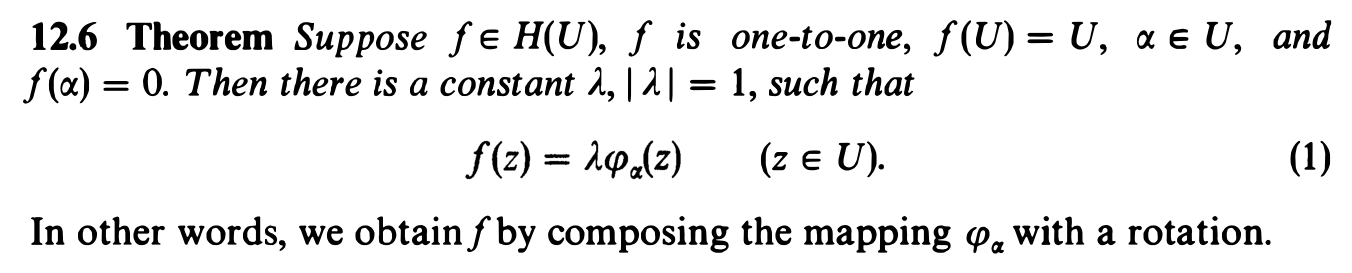
\includegraphics[width=\textwidth]{rudin-maximum-modulus-principle-2025052218.png}
% \caption{}
\label{}
\end{figure}

\begin{proof}
Let $g$ be the inverse of $f$, $f(g(z))=z$. As $f$ is injective, $f'(z)\neq0$,  $g'(z)=1/f'(z)$ exists for any $z\in U$, thus $g\in H(U)$. By the chain rule, $g'(0)f'(\alpha)=1$. By \cref{3725bc},
\[
\lvert f'(\alpha) \rvert \leq\frac{1-\lvert f(\alpha) \rvert ^2}{1-\lvert \alpha \rvert ^2} =\frac{1}{1-\lvert \alpha \rvert ^2}\qquad \lvert g'(0) \rvert \leq\frac{1-\lvert g(0) \rvert ^2}{1-0^2}=  1-\lvert \alpha \rvert ^2
\]
thus the equality holds. By \cref{0291fc}, with $\beta=0$, $f(z)=\lambda\varphi_{\alpha}(z)$ for some $\lvert \lambda \rvert=1$.
\end{proof}

\subsection{The Phragmen-Lindelof Method}

For unbounded regions, $\lVert f \rVert_{\Omega}=\lVert f \rVert_{\partial \Omega}$ for $f\in H(\Omega)$ is no longer true.

\begin{example}
Let $\Omega=\left\{  z=x+iy:-\frac{\pi}{2}<y<\frac{\pi}{2}  \right\}$, the boundary $\partial \Omega$ is $y=\pm \frac{\pi}{2}$. Put $f(z)=e^{ e^{ z } }$, for real $x$,
\[
f\left( x\pm\frac{\pi i}{2} \right)=\exp(\pm ie^{ x })
\]
$\lVert f \rVert_{\partial \Omega}=1$, but $\lVert f \rVert_{\Omega}=\infty$ since $\lim_{ x \to \infty }f(x)= \infty$.
\end{example}
\begin{theorem}
Suppose
\[
\Omega = \{x + iy : a < x < b\}, \quad \overline{\Omega} = \{x + iy : a \leq x \leq b\},
\]$f$ is continuous on $\overline{\Omega}$, $f \in H(\Omega)$, and suppose that $|f(z)| < B$ for all $z \in \Omega$ and some fixed $B < \infty$. If
\[
M(x) = \sup \{|f(x+iy)| : -\infty < y < \infty\} \quad (a \leq x \leq b)
\]then we actually have
\[
M(x)^{b-a} \leq M(a)^{b-x} M(b)^{x-a} \quad (a < x < b).
\]i.e. $\log M$ is a convex function on $(a,b)$.
\end{theorem}
\begin{proof}
WLOG, assume that $M(a)=M(b)=1$. Otherwise, replace $f$ by $\frac{f(x+iy)}{M(a)^{b-x}M(b)^{x-a}}$, which also satisfies the conditions, where $M(a)^{b-x}\coloneqq \exp \{ (b-x)\log M(a) \}$.

We need to show $\lvert f(z) \rvert\leq1$ for all $z\in \Omega$. For each $\epsilon>0$, define an auxiliary function
\[
h_{\epsilon}(z)=\frac{1}{1+\epsilon(z-a)}\qquad z\in \overline{\Omega}
\]
Since $\mathrm{Re}(1+\epsilon(z-a))=1+\epsilon(\text{Re }z-a)\geq1$, $\lvert h_{\epsilon} \rvert\leq1$ in $\overline{\Omega}$, thus $\lvert f (z) h_{\epsilon}(z) \rvert\leq1,\forall z\in \partial \Omega$. Also, $\lvert 1+\epsilon(z-a) \rvert\geq\epsilon \lvert y \rvert$, so that $\lvert f (z) h_{\epsilon}(z) \rvert\leq\frac{B}{\epsilon \lvert y \rvert},\forall z=x+iy\in \overline{\Omega}$.

Let $R_{\epsilon}$ be the rectangle cut off from $\overline{\Omega}$ by $y=\pm\frac{B}{\epsilon}$, then $\lvert fh_{\epsilon} \rvert\leq1$ on $\partial R_{\epsilon}$; hence on $R_{\epsilon}$ by the maximum modulus theorem.

For fixed $z\in \Omega$, $z\in R_{\epsilon}$ for any sufficiently small $\epsilon$, then $\lvert f(z)h_{\epsilon}(z) \rvert\leq1$; let $\epsilon\to0$, then $h_{\epsilon}\to1$, $\lvert f (z)\rvert\leq1$. We are done!
\end{proof}

\begin{figure}[H]
\centering
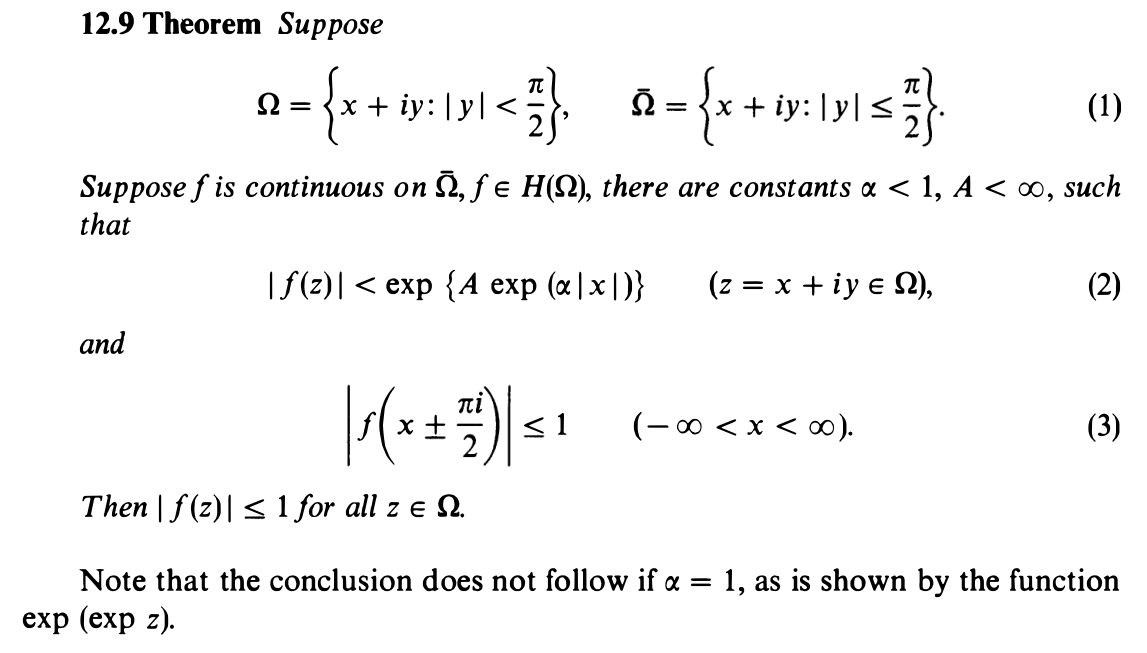
\includegraphics[width=\textwidth]{rudin-maximum-modulus-principle-2025052219.png}
% \caption{}
\label{}
\end{figure}

\subsection{A Converse of the Maximum Modulus Theorem}

The letter j will denote the identity function: $j(z) = z$. The function which assigns the number 1 to each $z \in U$ will be denoted by 1.

\begin{figure}[H]
\centering
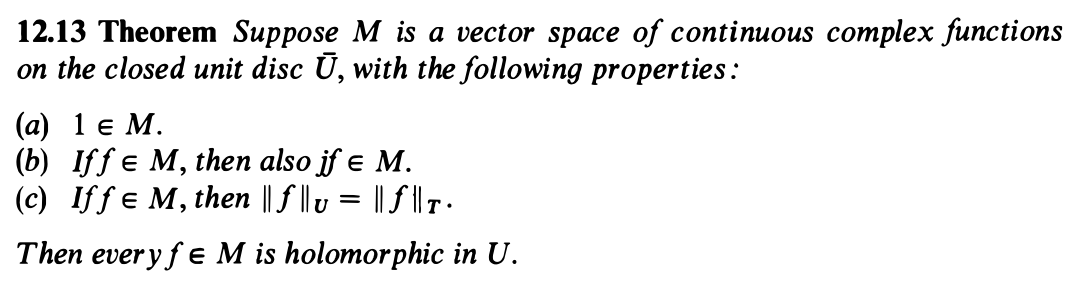
\includegraphics[width=\textwidth]{rudin-maximum-modulus-principle-2025052220.png}
% \caption{}
\label{}
\end{figure}

\begin{note}
Note that (c) is a rather weak form of the maximum modulus principle; (c) asserts only that the overall maximum of $|f|$ on $\bar{U}$ is attained at some point of the boundary $T$, but (c) does not a priori exclude the existence of local maxima of $|f|$ in $U$.
\end{note}
\begin{proof}
By (a) and (b), $M$ contains all polynomials. In conjunction with (c), this shows that $M$ satisfies the hypotheses of Theorem 5.25. Thus every $f\in M$ is harmonic in $U$. We shall use (b) to show that every $f\in M$ actually satisfies the Cauchy-Riemann equation.

Let $\partial$ and $\overline{\partial}$ be the differential operators introduced in Sec.11.1. The product rule for differentiation gives
\[
(\partial\overline{\partial})(fg)=f\cdot(\partial\overline{\partial}g)+(\partial f)\cdot(\overline{\partial}g)+(\overline{\partial}f)\cdot(\partial g)+(\partial\overline{\partial}f)\cdot g.
\]
Fix $f\in M$, and take $g=j$. Then $fj\in M$. Hence $f$ and $fj$ are harmonic, so $\partial\overline{\partial}f=0$ and $(\partial\overline{\partial})(f)=0$. Also, $\overline{\partial}j=0$ and $\partial j=1$. The above identity therefore reduces to $\overline{\partial}f=0$. Thus $f\in H(U)$.
\end{proof}
\begin{figure}[H]
\centering
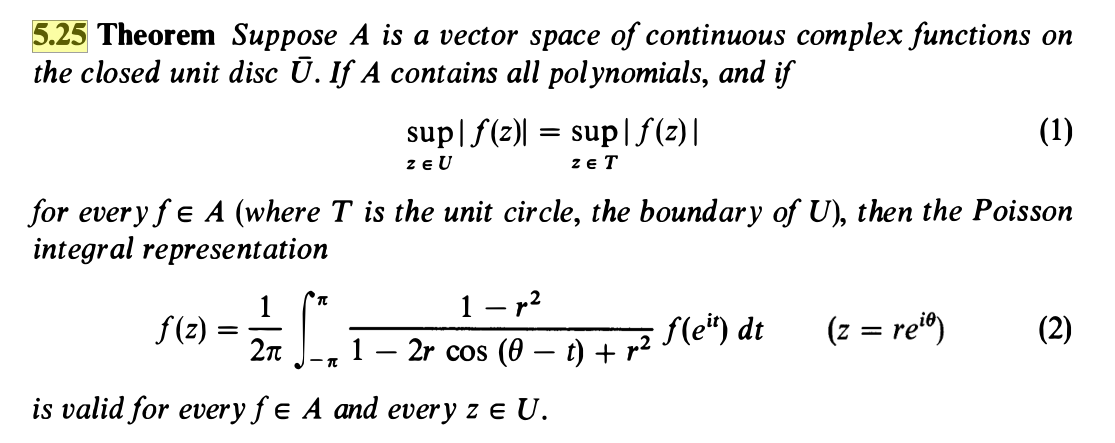
\includegraphics[width=\textwidth]{1-rudin-maximum-modulus-principle-2025052220.png}
% \caption{}
\label{}
\end{figure}

\begin{figure}[H]
\centering
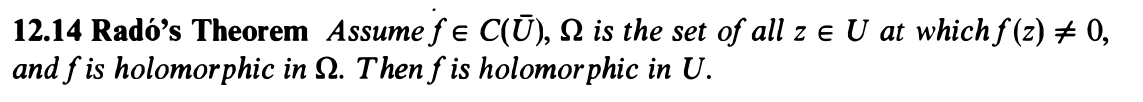
\includegraphics[width=\textwidth]{2-rudin-maximum-modulus-principle-2025052220.png}
% \caption{}
\label{}
\end{figure}

\begin{note}
In particular, the theorem asserts that $U-\Omega$ is at most countable, unless $\Omega=\varnothing$.
\end{note}
\subsection{Applications of Maximum Modulus Principle}

\begin{exercise}[Indiana]
Let $Q=[0,1] \times[0,1] \subset \mathbb{C}$ be the unit square, and let $f$ be holomorphic in a neighborhood of $Q$. Suppose that
\[
\begin{array}{ll}
f(z+1)-f(z) \text { is real and } \geq 0 & \text { for } z \in[0, i] \\
f(z+i)-f(z) \text { is real and } \geq 0 & \text { for } z \in[0,1]
\end{array}
\]Show that $f$ is constant.
\end{exercise}
\begin{proof}
Because $f$ is holomorphic on the closed unit square $Q$, by Cauchy integral theorem, we have
\[
\begin{aligned}
\int_{\partial Q} f(z) d z= & \int_0^1 f(x) d x+\int_0^1 f(1+y i) i d y-\int_0^1 f(x+i) d x -\int_0^1 f(y i) i d y \\
= & \int_0^1(f(x)-f(x+i)) d x+i \int_0^1(f(1+y i)-f(y i)) d y \\
= & 0
\end{aligned}
\]
As
\[
f(x)-f(x+i) \leq 0
\]
for $0 \leq x \leq 1$ and
\[
f(1+y i)-f(y i) \geq 0
\]
for $0 \leq y \leq 1$, by comparing the real and imaginary parts in the above identity, we obtain that $f(x+i)=f(x)$ for $0 \leq x \leq 1$ and $f(1+y i)=f(y i)$ for $0 \leq y \leq 1$. Hence $f(z)$ can be analytically extended to a double-periodic function by
\[
f(z)=f(z+1)=f(z+i)
\]
which is holomorphic in $\mathbb{C}$ and satisfies
\[
|f(z)| \leq \max _{z \in Q}\{|f(z)|\}<+\infty
\]
This shows that $f(z)$ must be a constant.
\end{proof}

\begin{exercise}
设 $f(z)$ 在区域 $0<|z|<1$ 内解析,$|f(z)|<\log \frac{1}{|z|}$ ,证明 $f(z) \equiv 0$ .
\end{exercise}
设 $g(z)=z f(z)$ ,由于 $f(z)$ 在 $0<|z|<1$ 内解析,$g(z)$ 在 $0<|z|<1$ 内也解析.
\[
|g(z)|=|z| \cdot|f(z)|<-|z| \cdot \ln |z|
\]
函数 $h(r)=-r \ln r$ 在 $(0,1)$ 上的最大值为 $\frac{1}{e}$ ,并且当 $r \rightarrow 0^{+}$或 $r \rightarrow 1^{-}$时,$h(r) \rightarrow 0$ .这说明 $g(z)$ 在该区域内有界的.

由于 $|g(z)| \rightarrow 0$ 当 $|z| \rightarrow 0^{+},|z| \rightarrow 1^{-}$.我们可以将 $g(z)$ 在 $z=0$ 处补定义 $g(0)=0$ ,从而 $g(z)$ 在单位圆盘 $|z|<1$ 内解析,并且 $|g(z)|<\frac{1}{e}$ .由于 $|g(z)| \rightarrow 0$ 当 $|z| \rightarrow 1^{-}$,根据最大模原理.$g(z) \equiv 0,0<|z|<1$ ,所以 $f(z) \equiv 0$ .
